\documentclass[12pt letter]{report}
\input{./template/preamble}
\input{./template/macros}
\input{./template/letterfonts}

\title{\Huge{Access Control}}
\author{\huge{Madiba Hudson-Quansah}}
\date{}
\usepackage{parskip}
\usepackage{tikz}
\usetikzlibrary{matrix}

\setcounter{tocdepth}{4}
\setcounter{secnumdepth}{4}

\begin{document}
\maketitle
\newpage
\pdfbookmark[section]{\contentsname}{too}
\tableofcontents
\pagebreak

\chapter{Introduction}

\dfn{Access Control}{
  The process of granting or denying specific requests to:
  \begin{itemize}
    \item Obtain and use information and related information processing services
    \item Enter specific physical facilities
  \end{itemize}
}

\dfn{Subject}{
  An entity capable of accessing objects. There are generally three classes:
  \begin{description}
    \item[Owner]  - The entity that has control over an object and can
      determine who has access to it.
    \item[Group] - A collection of users that share similar access needs.
    \item[World] - All other users not in the owner or group categories.
  \end{description}
}

\dfn{Object}{
  A resource to which access is controlled / An entity used to
  contain and/or receive information.
}

\dfn{Access Right}{
  Describes the way in which a subject may access and object. e.g.
  Read, Write, Execute.
}

Access control can be achieved through a combination of policies,
programs and technologies with the focus on the permission or
privileges that a subject has on an object.

\section{Access Control security Requirements (NIST SP 800-171)}

\chapter{Access Control Structures}

\section{Access Control Matrix (ACM)}

An abstract model that defines the rights of all subjects over all
objects in a system. It is represented as a matrix where:
\begin{itemize}
  \item Rows represent subjects.
  \item Columns represent objects.
  \item Each cell contains the access rights that the subject has over
    the object.
\end{itemize}
It is abstract because it cannot be feasibly implemented because:
\begin{itemize}
  \item The matrix can be very large and sparse.
  \item It is difficult to manage and update.
\end{itemize}
Example:
\begin{figure}[H]
  \centering
  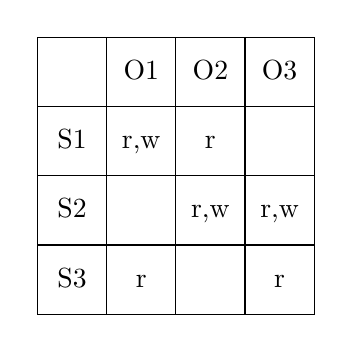
\begin{tikzpicture}
    \matrix (m) [matrix of nodes, nodes in empty cells,
      nodes={minimum width=2.5em, minimum height=2.5em,
        outer sep=0pt, anchor=center, text height=1.5ex,
      text depth=.25ex, draw},
    column sep=-\pgflinewidth, row sep=-\pgflinewidth] {
      & O1 & O2 & O3 \\
      S1 & r,w & r   &     \\
      S2 &     & r,w & r,w \\
      S3 & r   &     & r   \\
    };
  \end{tikzpicture}
\end{figure}

\section{Access Control List (ACL) / Capability List (CL)}

A more practical implementation of the ACM, where in the case of ACL,
each object has a list of subjects and their corresponding access
rights. This is commonly used in file systems. This is preferred when
there are more subjects than objects.
Example of ACL:
\begin{figure}[H]
  \centering
  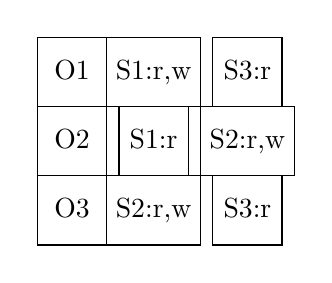
\begin{tikzpicture}
    \matrix (m) [matrix of nodes, nodes in empty cells,
      nodes={minimum width=2.5em, minimum height=2.5em,
        outer sep=0pt, anchor=center, text height=1.5ex,
      text depth=.25ex, draw},
    column sep=-\pgflinewidth, row sep=-\pgflinewidth] {
      O1 & S1:r,w & S3:r \\
      O2 & S1:r   & S2:r,w \\
      O3 & S2:r,w & S3:r \\
    };
  \end{tikzpicture}
\end{figure}

And in the case of CL, each subject has a list of objects and their
corresponding access rights. This is commonly used in
capability-based systems. This is preferred when there are more
objects than subjects.
Example of CL:
\begin{figure}[H]
  \centering
  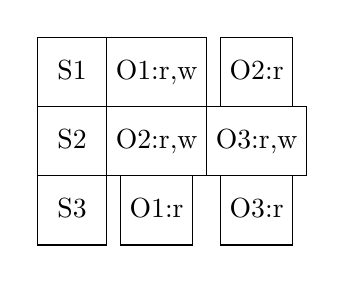
\begin{tikzpicture}
    \matrix (m) [matrix of nodes, nodes in empty cells,
      nodes={minimum width=2.5em, minimum height=2.5em,
        outer sep=0pt, anchor=center, text height=1.5ex,
      text depth=.25ex, draw},
    column sep=-\pgflinewidth, row sep=-\pgflinewidth] {
      S1 & O1:r,w & O2:r \\
      S2 & O2:r,w & O3:r,w \\
      S3 & O1:r   & O3:r \\
    };
  \end{tikzpicture}
\end{figure}

The main difference between ACL and CL is that ACL maps objects to
subject rights, but CL maps subjects to object rights.

\section{Authorization Table}
A table that defines the access rights of subjects to objects. It is commonly
used in access control systems such as Role-Based Access Control (RBAC) and
can include additional contextual attributes (e.g., time, location) similar to
Attribute-Based Access Control (ABAC).

\begin{table}[H]
  \centering
  \begin{tabular}{|c|c|c|c|}
    \hline
    \textbf{Subject} & \textbf{Object} & \textbf{Access Rights} &
    \textbf{Conditions} \\
    \hline
    S1 & O1 & r, w & 9am–5pm \\
    S2 & O2 & r & Location = A \\
    S3 & O3 & r, w & Location = B \\
    \hline
  \end{tabular}
\end{table}

\section{Extended Access Control Matrix (EACM)}

An extension of the ACM that includes additional contextual attributes
beyond just subjects, objects, and access rights. These attributes
can include conditions based on network addresses, protocols, port,
time of day and other criteria. Commonly used in network routers and
firewalls to control network traffic.
Example:
\begin{figure}[H]
  \centering
  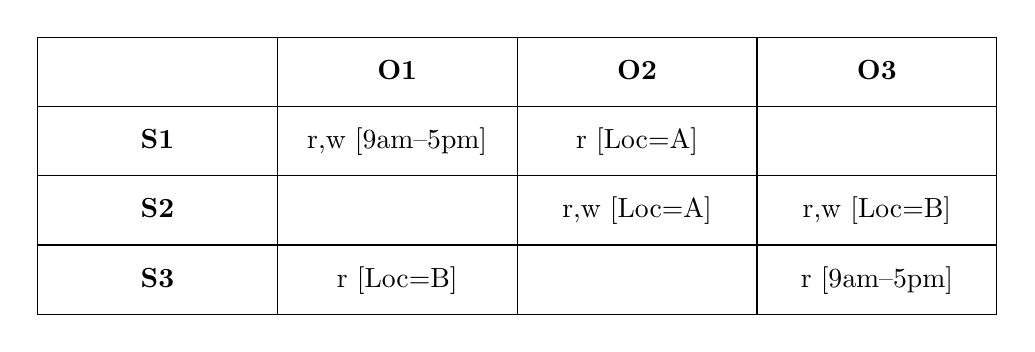
\begin{tikzpicture}
    \matrix (m) [
      matrix of nodes,
      nodes in empty cells,
      nodes={
        text width=8em,
        align=center,
        minimum height=2.5em,
        outer sep=0pt,
        anchor=center,
        text height=1.5ex,
        text depth=.25ex,
        draw
      },
      column sep=-\pgflinewidth,
      row sep=-\pgflinewidth
    ]{
      & \textbf{O1} & \textbf{O2} & \textbf{O3} \\
      \textbf{S1} & r,w [9am–5pm] & r [Loc=A] &  \\
      \textbf{S2} &  & r,w [Loc=A] & r,w [Loc=B] \\
      \textbf{S3} & r [Loc=B] &  & r [9am–5pm] \\
    };
  \end{tikzpicture}
\end{figure}

\chapter{Access Control Models}

\section{Discretionary Access Control (DAC)}
\dfn{Discretion}{
  The ability of an entity to determine who has access to its resources.
}

Provides the ability to share resources or information in a
peer-to-peer configuration, i.e. no centralized control. This allows
users to control and provide access to their own resources to others
at their discretion.

\section{Non-Discretionary Access Control (NDAC)}

Access control decisions are made by a central authority based on
predefined policies rather than individual user discretion. This
model is often used in environments where security and compliance are
critical.

\subsection{Mandatory Access Control (MAC)}

\dfn{Label}{
  A tag or marker that specifies the security level of an object or
  subject. e.g. Unclassified,  Confidential, Secret, Top Secret.
}

\begin{itemize}
  \item A system-enforced access rights are defined by a central
    policy not by users.
  \item Every subject and object has a security label.
\end{itemize}

\subsubsection{Rules}
Based on the Bell-LaPadula model:
\begin{description}
  \item[No Read Up] - Can't read higher classification, i.e. a user
    with "Secret" clearance cannot read "Top Secret" documents, but
    can read "Confidential" documents.
  \item[No Write Down] - Can't write to lower classification, i.e. a
    user with "Secret" clearance cannot write to "Confidential"
    documents, but can write to "Top Secret" documents.
\end{description}

\subsubsection{Goal}
\begin{itemize}
  \item Prevent information leakage between classification levels.
  \item  Protect confidentiality.
\end{itemize}

\subsubsection{Use cases}
\begin{itemize}
  \item Military Systems
  \item Government Agencies
  \item Critical Infrastructure
\end{itemize}

\subsection{Lattice-Based Access Control (LBAC)}
\begin{itemize}
  \item An extension of MAC that adds categories/compartments, i.e.
    modifiers to classification levels.
  \item Categories represent specific areas of information, e.g.
    Nuclear, Crypto, Finance, etc.
\end{itemize}

\subsubsection{Rules}
\begin{description}
  \item[Access is Allowed] - If the subject's security label/level is
    greater than or equal to the object's security label/level and
    the subject's categories include all of the object's categories, i.e.:
    \begin{align*}
      \text{Subject Level} \geq \text{Object Level} \wedge
      \text{Subject Categories} \supseteq \text{Object Categories}
    \end{align*}

\end{description}

\subsubsection{Goal}
\begin{itemize}
  \item Provides fine-grained control across multiple domains.
\end{itemize}

\subsubsection{Use cases}

\begin{itemize}
  \item Multi-Tenant cloud environments.
  \item Intelligence Agencies
  \item  Research
  \item Defence
\end{itemize}

\subsection{Role-Based Access Control (RBAC)}

\dfn{Role}{
  A collection of permissions that define a specific job function or
  responsibility within an organization.
}

RBAC assigns permission to specific roles within an organization.
Users are then assigned roles inheriting the permissions associated
with those roles. This model is based on the functions a user
performs within an organization simplifying access management.

\subsubsection{Rules}
\begin{description}
  \item[Role Assignment] - A user can only execute a role if they
    have been assigned to that role.
  \item[Role Authorization] - A user can only be assigned to roles
    for which they are authorized.
  \item[Permission Authorization] - A user can only exercise
    permissions that are authorized for their active role.
  \item[Role Hierarchies] - Roles can inherit permissions from other
    roles, allowing for a hierarchical structure of roles.
\end{description}

\subsubsection{Constraints}

\dfn{Constraint}{
  A defined relationship among roles, or a condition related to roles.
}

Constraints provide a means of adapting RBAC to the specifies of
administrative and security policies of an organization.

Types of constraints:
\begin{description}
  \item[Mutually Exclusive Roles] - A user can be assigned to one role in a set
    of roles but not to others in the same set. Any permission can be
    granted only one role in the set.
  \item[Cardinality] - Limits the maximum number of users that can be
    assigned to a specific role, or the maximum number of roles that can be
    assigned to a specific user.
  \item[Prequisite Roles] - Enforces that a user can only be assigned
    to a particular role if the user is already assigned to another
    specified role.
\end{description}

\subsection{Attribute-Based Access Control (ABAC)}

Access decisions are based on attributes of the user, rather than
roles or identities.
A policy defines rules that determine access based on these
attributes. This provides:
\begin{itemize}
  \item Fine-grained, context-aware access control
  \item More dynamic and scalable access management compared to RBAC
\end{itemize}

It is commonly used on cloud, government and zero-trust environments.

\end{document}
